\chapter{Experiment Description}

\section{The Large Hadron Collider (LHC)}
The Large Hadron Collider (LHC) is a high energy proton-proton collider that serves several modern particle physics detector experiments. 
Built at CERN and straddling the French-Swiss border, and first turned on for operation in 2008, it is the most powerful particle collider in history. 
The LHC was designed to collide protons at a maximum center of mass energy of $\sqrt s = 14\TeV$ 
with a maximum instantaneous luminosity of $10^{34}cm^{-2}s^{-1}$. To achieve this level of performance, the 27 km tunnel 
originally constructed for the Large Electron-Positron Collider (LEP) was repurposed to separately 
accelerate two couterrotating proton beams. The separate acceleration is made possible by oppositely oriented 
magnetic dipole fields in the two rings. When the beams achieve the desired energy, they are collided at one of four interaction points. 

The protons collided in the LHC are first gathered, bunched, and accelerated by other parts of the CERN accelerator complex before injection into the LHC ring. 
First, protons are stripped off of hydrogen atoms by a duoplasmatron and accelerated to 50\MeV by a linear accelerator (LINAC). Next, the protons are further accelerated 
in a series of synchroton rings of increasing size, the Proton Synchroton Booster (PSB), Proton Synchroton (PS), and Super Proton Synchroton (SPS). The SPS brings the 
proton beam energy up to 450\GeV. At this point, the beam is injected to the two LHC rings to be accelerated up to the final collision energy. Acceleration in the main 
ring is achieved by a system of thousands of superconducting dipole magnets, along with hundreds of correcting quadrupole magnets. A liquid helium cooling system is 
used to maintain the magnets at cryogenic temperatures. A full diagram of the CERN accelerator complex, including the parts relevant for the LHC, is shown in Fig. \ref{fig:accelerator_complex}.

\begin{figure}
  \centering
   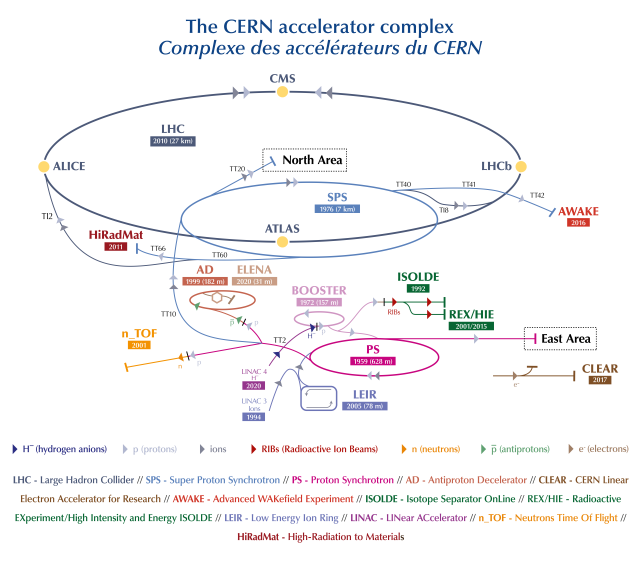
\includegraphics[width=0.9\textwidth]{fig/experiment/CCC-v2019-final-white.png}
	\caption{CERN accelerator complex.}
	\label{fig:accelerator_complex}
\end{figure}


\section{The Compact Muon Solenoid (CMS)}
The CMS apparatus~\cite{CMS:2008xjf} is a multipurpose, nearly hermetic detector, designed to trigger on~\cite{CMS:2020cmk,CMS:2016ngn} and identify electrons, muons, photons, and (charged and neutral) hadrons~\cite{CMS:2015xaf,CMS:2018rym,CMS:2015myp,CMS:2014pgm}.
The central feature of the CMS apparatus is a superconducting solenoid of 6\unit{m} internal diameter, providing a magnetic field of $3.8$\unit{T}. Within the solenoid volume are a silicon pixel and strip tracker, a lead tungstate crystal electromagnetic calorimeter (ECAL), and a brass and scintillator hadron calorimeter (HCAL), each composed of a barrel and two endcap sections. The ECAL consists of 75\,848 lead tungstate crystals, which provide coverage in pseudorapidity $\abs{\eta} < 1.48 $ in a barrel region (EB) and $1.48 < \abs{\eta} < 3.0$ in two endcap regions (EE). Preshower detectors consisting of two planes of silicon sensors interleaved with a total of $3$ radiation lengths of lead are located in front of each EE detector. Forward calorimeters extend the pseudorapidity coverage provided by the barrel and endcap detectors. Muons are measured in gas-ionization detectors embedded in the steel flux-return yoke outside the solenoid. A more detailed description of the detector components and operation is provided below. 
%A more detailed description of the CMS detector, together with a definition of the coordinate system used and the relevant kinematic variables, can be found in Ref.~\cite{CMS:2008xjf}.

\begin{figure}
  \centering
   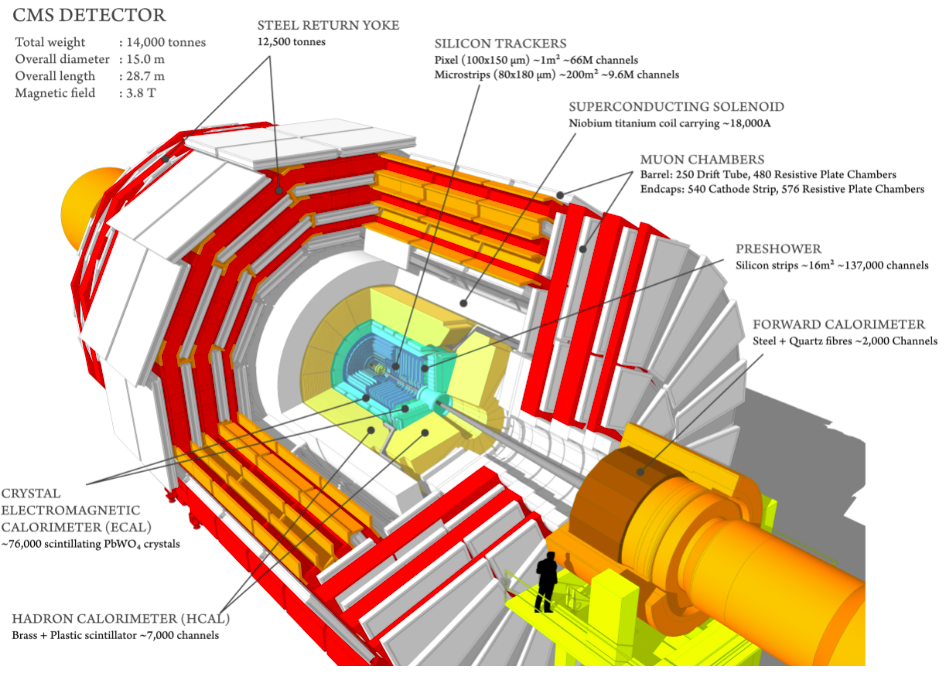
\includegraphics[width=0.9\textwidth]{fig/experiment/detector/cms_about_detector.png}
	\caption{The CMS detector apparatus.}
	\label{fig:detector}
\end{figure}


\subsection{Superconducting Magnet}
The function of the superconducting magnet within the CMS detector is to bend the trajectories of charged particles. This is crucial for particle identification and momentum measurement. 
Designed to provide a maximum magnetic field of $4$\unit{T}, its operating strength during pp collision runs is set to $3.8$\unit{T}. The bulk of the magnet is composed of NbTi, cooled by 
liquid helium to 4.5K, which is below the critical temperature allowing for superconductivity. The magnet has a length of 12.5m, diameter of 6.3m, and mass of 220 tons. The solenoid encloses 
several detector components, including the tracker and the majority of the calorimeters. A steel flux-return yoke is built around the solenoid, and is composed of 5 wheels and two endcaps weighing 
a total of roughly 10,000 tons. 

\subsection{Inner Tracking System}
The inner tracking system is designed to reconstruct charged particle trajectories and vertices arising from particle decays. Comprised of a silicon pixel detector and silicon strip tracker, 
it covers the pseudorapidity region $|\eta| < 2.5$ and is designed for efficient and precise measurement of charged particles with \pt about about 1\GeV. 
At the LHC design luminosity for pp collisions, each bunch crossing leads to about 1,000 hits in the inner tracking system. As such, the inner tracking system was designed to be 
maximally radiation tolerant while maintaining physics performance. 

The silicon pixel detector covers the inner region of $r < 10 cm$. It is composed of $100 \times 150 \mu m^{2}$ pixels arranged in three barrel layers and two endcap disks. Due to the extreme 
radiation environment, the innermost layer was designed to be replaced after at least two years of LHC operation. 
In response to LHC running conditions and detector degradation, a replacement and upgrade of the full pixel detector was made during the LHC extended year-end technical stop in 2016/2017. 
The silicon strip tracker covers the region $20 < r < 116 cm$. It is divided into three subsystems: the Tracker Inner Barrel (TIB), Tracker Inner Disks (TID), and Tracker Outer Barrel (TOB). 
The strip thickness is $320 \mu m$ ($500 \mu m$) in the TIB/TID (TOB). A schematic diagram of the CMS inner tracking system in the r-z plane is shown in Fig. \ref{fig:cms_tracker}.

\begin{figure}
  \centering
   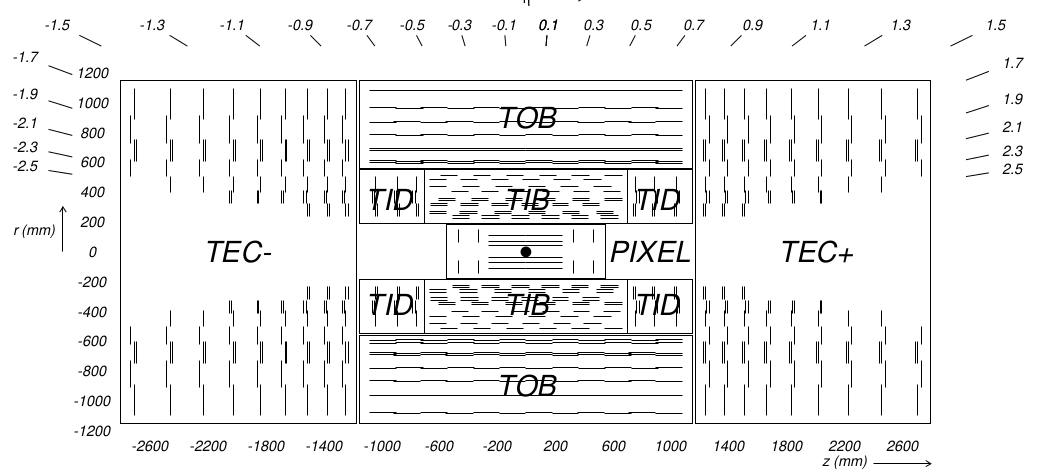
\includegraphics[width=0.9\textwidth]{fig/experiment/detector/cms_tracker.png}
	\caption{Cross section of the CMS inner tracking system in the r-z plane.}
	\label{fig:cms_tracker}
\end{figure}


\subsection{Electromagnetic Calorimeter (ECAL)}

\subsection{Hadronic Calorimeter (HCAL)}

\subsection{Muon Detectors}

\begin{figure}
  \centering
   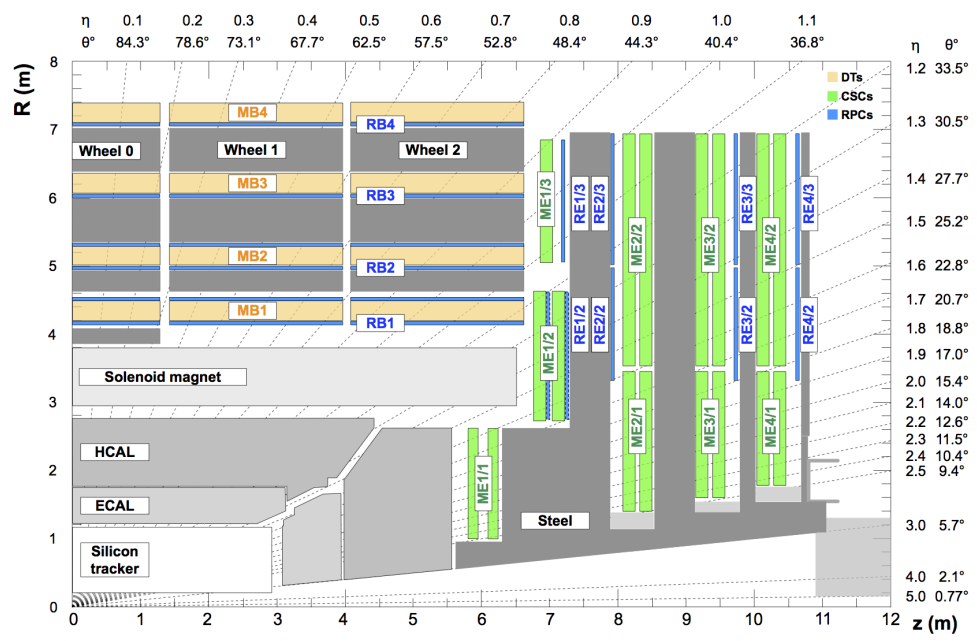
\includegraphics[width=0.9\textwidth]{fig/experiment/detector/muon_sys_r-z.png}
	\caption{Diagram of CMS detector in the r-z plane showing the components of the muon system.}
\end{figure}

\section{Trigger System}

\section{Object Reconstruction}
The global event reconstruction (also called particle-flow (PF) event reconstruction~\cite{CMS:2017yfk}) aims to reconstruct and identify each individual particle in an event, with an optimized combination of all subdetector information. In this process, the identification of the particle type (photon, electron, muon, charged hadron, neutral hadron) plays an important role in the determination of the particle direction and energy.

\begin{figure}
  \centering
   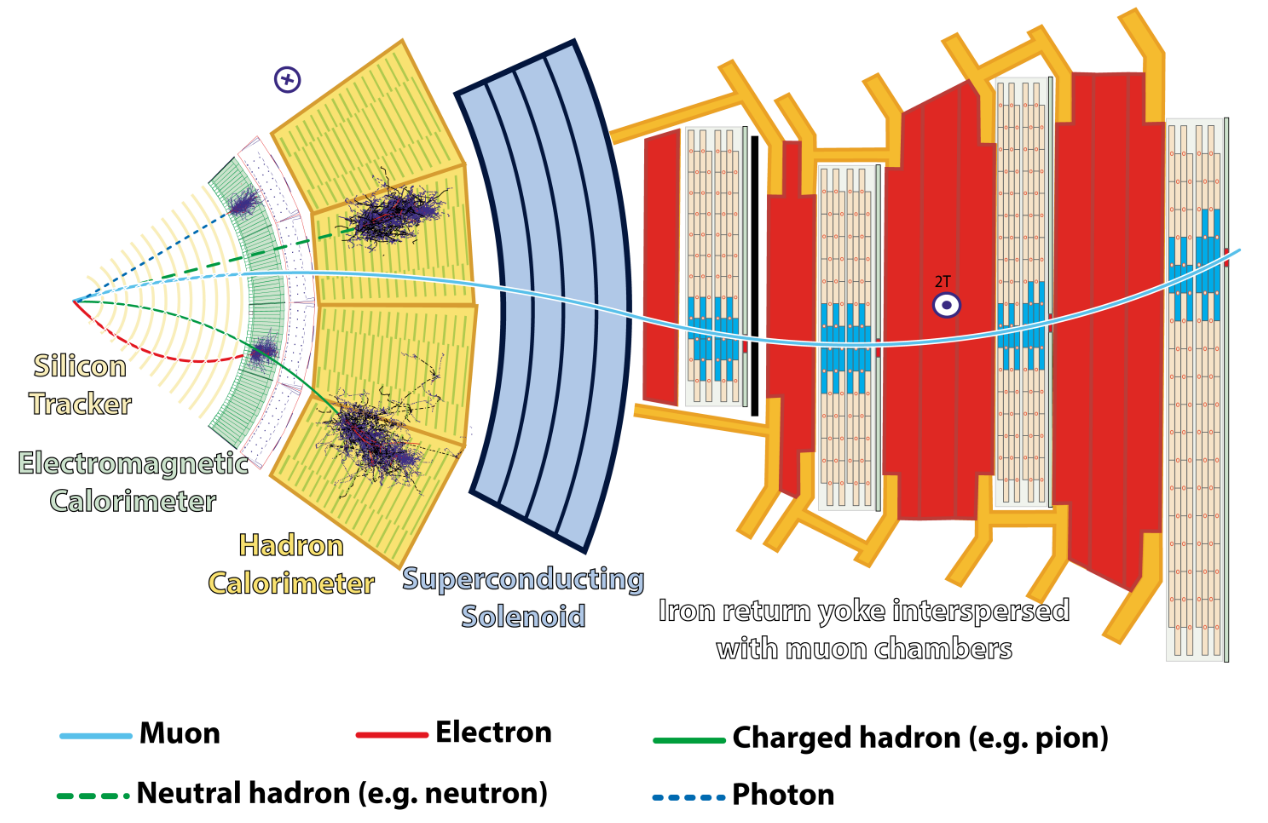
\includegraphics[width=0.9\textwidth]{fig/experiment/reconstruction/cms_detector.png}
	\caption{Schematic of different particles interacting with the CMS detector.}
\end{figure}

\subsection{Photon and Electron Reconstruction}
Photons and electrons interact with the material in the ECAL, depositing the majority of their energy before reaching the HCAL. As they interact, photons convert into 
electron-positron pairs and electrons radiate bremsstrahlung photons. This leads to the formation of an electromagnetic shower. Because of this, the original particle energy 
is split into multiple energy deposits, which must be combined to reconstruct the original energy. Deposits in individual ECAL crystals are combined into clusters, 
and these clusters are in turn combined into superclusters. Two algorithms are used to generate superclusters: the so-called "mustache" algorithm, and the so-called "refined" algorithm.
The mustache algorithm defines a seed cluster with energy above a certain threshold, and then combines it with other clusters within a region of the eta-phi plane centered at the 
seed location. The refined algorithm uses the mustache superclusters as well as tracking information to extrapolate bremsstrahlung and conversion tracks to decide whether a cluster should belong 
to the supercluster. 

The distinction between photons and electrons is made using tracking information, where photons are associated with no tracks and electrons with tracks. The Gaussian Sum Filter (GSF) [REF] track 
fitting algorithm is used to identify and characterize tracks that might be associated with an electron. It first begins with a hit pattern in the tracker, which is used as a seed. This seed 
can either be tracker-driven, coming from the collection of generic tracks tested for mutual compatibility, or it can be ECAL-driven, where a mustache supercluster is compared in location with 
a collection of tracker hit patterns to determine if the supercluster is consistent with the trajectory indicated by the track. Electron seeds are then converted into reconstructed electron tracks. 
In the absence of any GSF electron tracks, a photon candidate is obtained. Additional separation between photons and electrons is obtained through further selection requirements. 
The measured energy resolution for electrons produced in $\PZ$ boson decays in  $\Pp\Pp$ collision data ranges from $2$--$5$\%, depending on electron pseudorapidity and energy loss through bremsstrahlung in the detector material~\cite{CMS:2020uim}.

\subsection{Muon Reconstruction}
Muon reconstruction utilizes information from the muon detectors and the tracker. First, detector hits in the CSCs, DTs, and RPCs are used to build standalone tracks using a Kalman-filter technique.
Subsequently, these standalone muon tracks are combined with tracker information via two algorithms. So-called "tracker muons" are reconstructed using an "inside-out" algorithm, which starts from 
tracker tracks and matches them to DT or CSC segments. So-called "global muons" are reconstructed with an "outside-in" approach which starts from standalone muon tracks and matches them 
to tracker tracks using a Kalman-filter technique. In the case where both algorithms reconstruct a muon sharing the same tracker tack, the two outputs are merged into a single muon candidate.
In general, the tracker muon algorithm is more efficient in the region of low muon \pT, while the global algorithm is efficient at high \pT. 

The energy of muons is obtained from the corresponding track momentum. Matching muons to tracks measured in the silicon tracker results in a \pt resolution, for muons with \pt up to $100$\GeV, of $1$\% in the barrel and $3$\% in the endcaps. The \pt resolution in the barrel is better than $7$\% for muons with \pt up to $1$\TeV~\cite{CMS:2018rym}.


\subsection{Hadrons}
Charged hadrons are identified as charged particle tracks that are neither identified as electrons nor as muons. Neutral hadrons are identified as HCAL energy clusters not linked to any charged hadron trajectory, or as a combined ECAL and HCAL energy excess with respect to the expected charged hadron energy deposit.

\subsection{Jets}

\begin{figure}
  \centering
   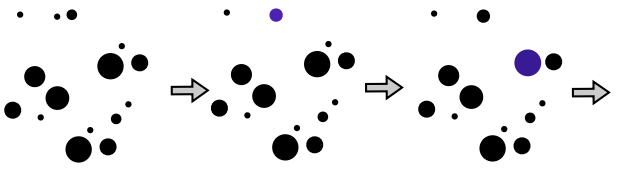
\includegraphics[width=0.9\textwidth]{fig/experiment/reconstruction/jet_clustering.png}
	\caption{Diagram representing the jet clustering algorithm.}
\end{figure}

\subsection{Primary Vertex}
